\documentclass{article}
\usepackage{enumerate}
\usepackage{amsmath}
\usepackage{amssymb}
\usepackage{graphicx}
\usepackage{subfigure}
\usepackage{geometry}
\usepackage{color}
\usepackage{bm}
\usepackage{indentfirst}
\usepackage{float}
\usepackage{booktabs}

\begin{document}

\vspace*{0.25cm}

\hrulefill

\thispagestyle{empty}

\begin{center}
\begin{large}
\sc{UM--SJTU Joint Institute \vspace{0.3em} \\ Physics Laboratory \\(VP241)}
\end{large}

\hrulefill

\vspace*{5cm}
\begin{Large}
\sc{{Laboratory Report}}
\end{Large}

\vspace{2em}

\begin{large}
\sc{{Exercise 2
\vspace{0.5em}

The Hall Probe: Characteristics and Applications
}}
\end{large}
\end{center}


\vfill

\begin{table}[h!]
\flushleft
\begin{tabular}{lll}
Name: Yihao Liu \hspace*{2em}&
ID: 515370910207\hspace*{2em} \\
Name: Guangzheng Wu \hspace*{2em}&
ID: 515370910175\hspace*{2em}& Group: 7\\


\\

Date: 21 Oct 2016 

\end{tabular}
\end{table}

\hfill
\begin{tiny}
[rev. 1.0]
\end{tiny}

\newpage

\tableofcontents

\newpage

\section{Objectives}

In 1879 E.H. Hall observed that when an electric current passes through a sample placed in a magnetic field, electric potential difference proportional to the current and to the magnetic field appears across the material in the direction perpendicular to both the current and the magnetic field. This effect is known as the Hall effect, and since its discovery it has found many practical applications. The principle of the Hall effect is used in devices for magnetic field measurements as well as in position and motion detectors.\\

The objective of this exercise is to study the principle of the Hall effect and its applications by  using a Hall probe.  In particular, it will be verified that the Hall voltage is proportional to the magnetic field. Furthermore, the sensitivity of an integrated Hall probe will be studied by calculating the magnetic field at the center of a solenoid, and the magnetic field distribution along the axis of the solenoid will be measured and compared with the corresponding theoretical curve.

\section{Theoretical Background}

\subsection{Hall Effect}

Consider a conducting sheet (made of a metal or a semiconductor) placed in a magnetic   field so that the plane of the sheet is perpendicular to the direction of the magnetic field B (Figure 1).  When the electric current I passes through the sheet in the direction shown in Figure 1, an electric potential difference between the sides a and b of the sheet is generated. The corresponding electric field is perpendicular to both the direction of the current and the direction of the magnetic field. This effect is known as the Hall effect, and the electric potential difference is called the Hall voltage $U_H$.

\begin{figure}[H]
	\centering
	\includegraphics[scale=0.6]{p1.png}
	\caption{The principle of the Hall effect.}
\end{figure}

Microscopically, the Hall effect is caused by the Lorentz force, that is a force acting on charges moving in a magnetic field. The Lorentz force $ F_B $ leads to the deflection of the moving charges, and their accumulation on one side of the sheet, which in turn increases the magnitude of the transverse electric field $ E_H $. Due to this field, there is an electric force $ F_E $ acting upon the charges, and since $ F_B $ and $ F_E $ act in opposite directions, a balance is eventually reached and $ U_H $ stabilizes.

When the external magnetic field is not too strong, the Hall voltage is proportional to both the current and the magnitude of the magnetic field, and inversely proportional to the thickness of the sheet $ d $

\begin{equation}
U_H=R_H\dfrac{IB}{d}=KIB
\end{equation}


where $ R_H $ is the so-called Hall coefficient and $ K=R_H/d=K_H/I $, where $ K_H $ is the so-called sensitivity of the Hall element.

\subsection{Integrated Hall Probe}
The magnitude of the magnetic field can be found by measuring the Hall voltage with a Hall probe when the sensitivity $ K_H $ and the current I are fixed. Since the Hall voltage is usually very small, it should be amplified before the measurement.

Silicon can be used to design both the Hall probe and the integrated circuits, so it is convenient to arrange the Hall probe and the electric circuits into a single device. Such a device is called an integrated Hall probe.

The integrated Hall probe SS495A consists of a Hall sensor, an amplifier, and a voltage compensator (Figure 2). The output voltage U can be read ignoring the residual voltage. The working voltage $ U_S = 5 V $, and the output voltage $ U_0 $ is approximately $ 2.5 V $ when the magnetic field is zero. The relation between the output voltage U and the magnitude of the magnetic field is
\begin{equation}
	B=\dfrac{U-U_0}{K_H}
\end{equation}
\begin{figure}[H]
	\centering
	\includegraphics[scale=0.6]{p2.png}
	\caption{The integrated Hall probe SS495A (left). The relation between the output voltage $ U $ and the magnitude of the magnetic field $ B $ (right).}
\end{figure}

\subsection{Magnetic Field Distribution Inside a Solenoid}

The magnetic field distribution on the axis of a single layer solenoid can be calculated from the following formula
\begin{equation}
	B(x)=\mu_0\dfrac{N}{L}I_M\begin{Bmatrix}
	\dfrac{L+2x}{2[D^2+(L+2x)^2]^{\frac{1}{2}}}+\dfrac{L-2x}{2[D^2+(L-2x)^2]^{\frac{1}{2}}}
	\end{Bmatrix}=C(x)I_M
\end{equation}
where $ N $ is the number of turns of the solenoid, $ L $ is its length, $ I_M $ is the current through the solenoid wire, and $ D $ is the solenoid's diameter. The magnetic permeability of vacuum is $ \mu_0=4\pi\times10^{-7}H/m $

The solenoid used in this exercise has ten layers, and the magnetic field $ B(x) $ for each layer can be calculated using Eq. (3). Then the net magnetic on the axis of the solenoid can be found by adding contributions due to all layers. The theoretical value of the magnetic field inside the solenoid with $ I_M = 0.1 A $ is given in Table 1.
\begin{table}[H]
	\centering
	\begin{tabular}{|c|c||c|c|}
		\hline
		x[cm]     & B[mT]      &    x[cm]   & B[mT] \\
		\hline
		$ \pm $0.0     & 1.4366  & $\pm$8.0     & 1.4057  \\
		$\pm$1.0     & 1.4363  & $\pm$9.0     & 1.3856  \\
		$\pm$2.0     & 1.4356  & $\pm$10.0    & 1.3478  \\
		$\pm$3.0     & 1.4343  & $\pm$11.0    & 1.2685  \\
		$\pm$4.0     & 1.4323  & $\pm$11.5  & 1.1963  \\
		$\pm$5.0     & 1.4292  & $\pm$12.0    & 1.0863  \\
		$\pm$6.0     & 1.4245  & $\pm$12.5  & 0.9261  \\
		$\pm$7.0     & 1.4173  & $\pm$13.0    & 0.7233  \\
		\hline
	\end{tabular}
	\caption{Theoretical value of the magnetic field inside the solenoid.}
\end{table}


\section{Measurement Setup and Procedure}

\subsection{Apparatus}

The experimental setup shown in Figure 5 consists of an integrated Hall probe SS495A (see Figure 4) with $ K_H = 31.25 \pm 1.25 V/T $ or $ K_H = 3.125 \pm 0.125 mV/G $, a solenoid, a power supply, a voltmeter, a DC voltage divider, and a set of connecting wires.
\begin{figure}[H]
	\centering
	\includegraphics[scale=0.6]{p3.png}
	\caption{Measurement setup.}
\end{figure}
\begin{figure}[H]
	\centering
	\includegraphics[scale=0.6]{p4.png}
	\caption{Integrated Hall probe SS495A.}
\end{figure}

\subsection{Measurement Procedure}

\subsubsection{Relation Between Sensitivity $ K_H $ and Working Voltage $ U_S $}
\begin{enumerate}
	\item Place the integrated Hall probe at the center of the solenoid. Set the working voltage at 5 V and measure the output voltage $ U_0 (I_M = 0) $ and $ U (I_M = 250 mA) $. Take the theoretical value of $ B(x = 0) $ from Table 1 and calculate the sensitivity of the probe $ K_H $ by using Eq. (2).\
	\item Measure $ K_H $ for different values of $ U_S $ (from $ 2.8 V $ to $ 10 V $). Calculate $ K_H/U_S $ and plot the curve $ K_H/U_S vs. U_S $.
\end{enumerate}
\subsubsection{Relation Between Output Voltage $ U $ and Magnetic Field $ B $}
\begin{enumerate}
	\item With $ B=0, U_S=5 V, $ connect the $ 2.4 \sim 2.6 V $ output terminal of the DC voltage divider and the negative port of the voltmeter. Adjust the voltage until $ U_0 = 0 $.
	\item Place the integrated Hall probe at the center of the solenoid and measure the output voltage $ U $ for different values of $ I_M $ ranging from 0 to $ 500 mA $, with intervals of $ 50 mA $.
	\item Explain the relation between $ B(x = 0) $ and the Hall voltage $ U_H $. Pay attention to the fact that the output voltage U is the amplified signal from $ U_H $. The theoretical value of $ B(x = 0) $ can be found from Table 1.
	\item Plot the curve $ U vs. B $ and find the sensitivity $ K_H $ by a linear fit (use a computer). Compare the value you obtained with the theoretical value in given in the Apparatus section.
\end{enumerate}
\subsubsection{Magnetic Field Distribution Inside the Solenoid}
\begin{enumerate}
	\item Measure the magnetic field distribution along the axis of the solenoid for $ I_M = 250 mA $, record the output voltage U and the corresponding position $ x $. Then find $ B = B(x) $. (Use the value of $ K_H $ found in the previous part of the experiment).
	\item Use a computer to plot the theoretical and the experimental curve showing the magnetic field distribution inside the solenoid. Use dots for the data measured and a solid line for the theoretical curve. The origin of the plot should be at the center of the solenoid.
\end{enumerate}

\section{Results}


\subsection{Relation Between Sensitivity $ K_H $ and Working Voltage $ U_S $}

The measurement of $U$ was shown in Table \ref{tab-1}.

\begin{table}[!h]
\begin{center}
\begin{tabular}{|c|c|c|}
\hline
$U_S$ [V] $\pm$ 0.5\% V & $U_0(I_M=0)$ [V] $\pm$ $0.5\% +6\times10^{-3}$ V  &
$U_0(I_M=250mA)$ [V] $\pm$ $0.5\% +6\times10^{-3}$ V\\
\hline
5.00 & 2.588 & 2.696\\
\hline
\end{tabular}
\caption{Data for $U_0$ and $U$ with $U_S=5V$.}
\label{tab-1}
\end{center}
\end{table}

Then we can calculate $K_H$

$$K_H=\frac{U-U_0}{B}=\frac{2.696-2.588}{2.5\cdot1.4366\times10^{-3}}=30.071\pm2.882\,\rm{V/T}$$

The measurement of different $U$ was shown in Table \ref{tab-2}.

\begin{table}[!h]
\begin{center}
\begin{tabular}{|c|c|c|c|}
\hline
&$U_S$ [V] $\pm$ 0.5\% V & $U_0$ [V] $\pm$ $0.5\% +6\times10^{-3}$ V &$U_0$ [V] $\pm$ $0.5\% +6\times10^{-3}$ V\\
\hline
1	&	2.77	&	1.4958	&	1.5433	\\
\hline
2	&	3.25	&	1.6613	&	1.7254	\\
\hline
3	&	3.78	&	1.9408	&	2.0198	\\
\hline
4	&	4.24	&	2.185	&	2.276	\\
\hline
5	&	4.77	&	2.463	&	2.566	\\
\hline
6	&	5.26	&	2.722	&	2.837	\\
\hline
7	&	5.77	&	2.988	&	3.115	\\
\hline
8	&	6.27	&	3.252	&	3.391	\\
\hline
9	&	6.73	&	3.492	&	3.641	\\
\hline
10	&	7.27	&	3.773	&	3.932	\\
\hline
11	&	7.76	&	4.030	&	4.200	\\
\hline
12	&	8.26	&	4.291	&	4.473	\\
\hline
13	&	9.39	&	4.877	&	5.084	\\
\hline
14	&	9.90	&	5.146	&	5.362	\\
\hline
\end{tabular}

\caption{Data for $U_0$ and $U$ with $U_S=5V$.}
\label{tab-2}
\end{center}
\end{table}

Then we can calculate $K_H$ and $K_H/U_S$ in in Table \ref{tab-2-2}.

\begin{table}[!h]
\begin{center}
\begin{tabular}{|c|c|c|}
\hline
& $K_H$ [V/T] & $K_H/U_S$ [1/T] \\
\hline
1	&	$13.226\pm2.662$	&	$4.775\pm0.961$	\\
\hline
2	&	$17.848\pm2.696$	&	$5.492\pm0.830$	\\
\hline
3	&	$21.996\pm2.753$	&	$5.819\pm0.728$	\\
\hline
4	&	$25.338\pm2.802$	&	$5.976\pm0.661$	\\
\hline
5	&	$28.679\pm2.858$	&	$6.012\pm0.599$	\\
\hline
6	&	$32.020\pm2.910$	&	$6.087\pm0.553$	\\
\hline
7	&	$35.361\pm2.963$	&	$6.128\pm0.514$	\\
\hline
8	&	$38.702\pm3.017$	&	$6.173\pm0.481$	\\
\hline
9	&	$41.487\pm3.065$	&	$6.164\pm0.455$	\\
\hline
10	&	$44.271\pm3.121$	&	$6.090\pm0.429$	\\
\hline
11	&	$47.334\pm3.173$	&	$6.100\pm0.409$	\\
\hline
12	&	$50.675\pm3.225$	&	$6.135\pm0.390$	\\
\hline
13	&	$57.636\pm3.343$	&	$6.138\pm0.356$	\\
\hline
14	&	$60.142\pm3.397$	&	$6.075\pm0.343$	\\
\hline
\end{tabular}

\caption{$K_H$ and $K_H/U_S$.}
\label{tab-2-2}
\end{center}
\end{table}

The curve $U_S$ vs. $K_H/U_S$ was plotted in Figure \ref{fig-1}.

\begin{figure}[H]
	\centering
	\includegraphics[scale=0.6]{fig1.eps}
	\caption{$U_S$ vs. $K_H/U_S$.}
	\label{fig-1}
\end{figure}

\newpage


\subsection{Relation Between Output Voltage $ U $ and Magnetic Field $ B $}

The measurement of $U$ was shown in Table \ref{tab-3}.

\begin{table}[!h]
\begin{center}
\begin{tabular}{|c|c|c|}
\hline
& $I_M$ [mA] $\pm$ 2\% [mA] & $U$ [V] $\pm$ $0.05\%+6\times10^{-3}$ [V] \\
\hline
1	&	0.000	&	0.000	\\
\hline
2	&	50.000	&	0.021	\\
\hline
3	&	100.000	&	0.043	\\
\hline
4	&	150.000	&	0.065	\\
\hline
5	&	200.000	&	0.086	\\
\hline
6	&	250.000	&	0.109	\\
\hline
7	&	300.000	&	0.130	\\
\hline
8	&	350.000	&	0.152	\\
\hline
9	&	400.000	&	0.174	\\
\hline
10	&	450.000	&	0.196	\\
\hline
11	&	500.000	&	0.217	\\
\hline
\end{tabular}

\caption{Measurement data for the $I_M$ vs. $U$ relation.}
\label{tab-3}
\end{center}
\end{table}

$$B=\frac{U}{K_H}=\frac{kU_H}{K_H}$$

Then we can make a plot of $U$ vs. $B$ and find $K_H$, it was shown in Figure \ref{fig-2}.

\begin{figure}[H]
	\centering
	\includegraphics[scale=0.6]{fig2.eps}
	\caption{$U$ vs. $B$.}
	\label{fig-2}
\end{figure}

So $K_H=30.2874\pm0.00017\,\rm{V/T}$

\subsection{Magnetic Field Distribution Inside the Solenoid}

The measurement of $U$ was shown in Table \ref{tab-4}.

\begin{table}[!h]
\begin{center}
\begin{tabular}{|c|c|c||c|c|c|}
\hline
&$x$[cm]$\pm$0.05[cm]&$U$[V]$\pm0.05\%+6\times10^{-4}$[V]& &$x$[cm]$\pm$0.05[cm]&$U$[V]$\pm0.05\%+6\times10^{-4}$[V] \\
\hline
1	&	0.00	&	1.7565	&	25	&	14.40	&	3.5890	\\
\hline
2	&	0.60	&	2.3970	&	26	&	15.00	&	3.5890	\\
\hline
3	&	1.20	&	2.8263	&	27	&	15.60	&	3.5856	\\
\hline
4	&	1.80	&	3.0970	&	28	&	16.20	&	3.5823	\\
\hline
5	&	2.40	&	3.2621	&	29	&	16.80	&	3.5790	\\
\hline
6	&	3.00	&	3.3578	&	30	&	17.40	&	3.5790	\\
\hline
7	&	3.60	&	3.4239	&	31	&	18.00	&	3.5724	\\
\hline
8	&	4.20	&	3.4668	&	32	&	18.60	&	3.5658	\\
\hline
9	&	4.80	&	3.4965	&	33	&	19.20	&	3.5559	\\
\hline
10	&	5.40	&	3.5196	&	34	&	19.80	&	3.5460	\\
\hline
11	&	6.00	&	3.5328	&	35	&	20.40	&	3.5262	\\
\hline
12	&	6.60	&	3.5460	&	36	&	21.00	&	3.5097	\\
\hline
13	&	7.20	&	3.5559	&	37	&	21.60	&	3.4899	\\
\hline
14	&	7.80	&	3.5658	&	38	&	22.20	&	3.4536	\\
\hline
15	&	8.40	&	3.5724	&	39	&	22.80	&	3.4008	\\
\hline
16	&	9.00	&	3.5757	&	40	&	23.40	&	3.3248	\\
\hline
17	&	9.60	&	3.5790	&	41	&	24.00	&	3.1927	\\
\hline
18	&	10.20	&	3.5790	&	42	&	24.60	&	2.9715	\\
\hline
19	&	10.80	&	3.5823	&	43	&	25.20	&	2.6282	\\
\hline
20	&	11.40	&	3.5823	&	44	&	25.80	&	2.0768	\\
\hline
21	&	12.00	&	3.5823	&	45	&	26.40	&	1.4461	\\
\hline
22	&	12.60	&	3.5823	&	46	&	27.00	&	0.9311	\\
\hline
23	&	13.20	&	3.5856	&	47	&	27.60	&	0.5976	\\
\hline
24	&	13.80	&	3.5856	&	&	&	\\
\hline
\end{tabular}

\caption{Data for he $U$ vs. $x$ relation.}
\label{tab-4}
\end{center}
\end{table}

The theoretical and the experimental curve showing the magnetic field distribution inside the solenoid was shown in Figure \ref{fig-3}.

\begin{figure}[H]
	\centering
	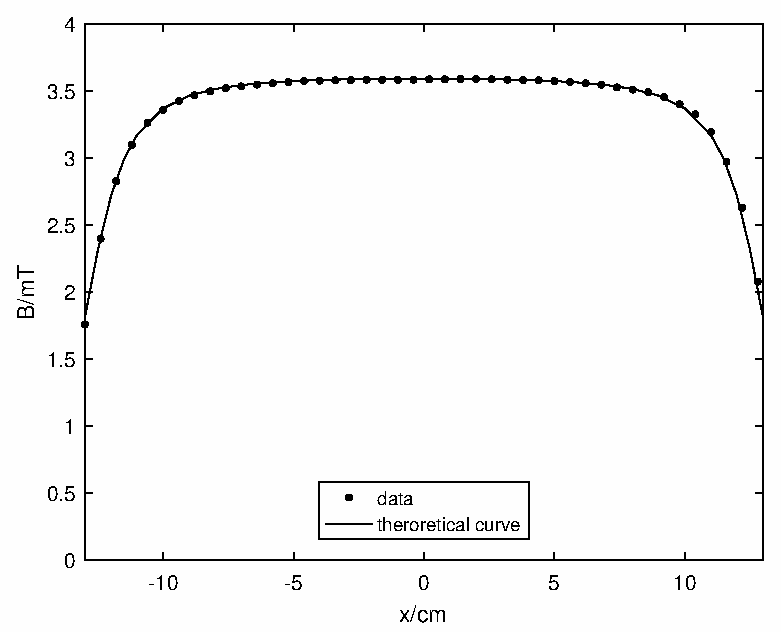
\includegraphics[scale=0.6]{fig3.eps}
	\caption{$B(x)$.}
	\label{fig-3}
\end{figure}

\newpage

\section{Measurement uncertainty analysis}

\subsection{Relation Between Sensitivity $ K_H $ and Working Voltage $ U_S $}

$K_H$ can be calculated by the equation $K_H=\frac{U-U_0}{B}$. Therefore its uncertainty $u_{K_H}$ is found by applying the uncertainty propagation formula

\begin{align*}
u_{K_H}&=\sqrt{\left(\frac{\partial K_H}{\partial U}\right)^2u_U^2+\left(\frac{\partial K_H}{\partial U_0}\right)^2u_{U_0}^2}\\
&=\sqrt{\left(\frac{1}{B}\right)^2u_U^2+\left(\frac{1}{B}\right)^2u_{U_0}^2}\\
&=2.882\,\rm{V/T}
\end{align*}

So $K_H=30.071\pm2.882\,\rm{V/T}$\\

The uncertainty $u_{K_H/U_S}$ is found by applying the uncertainty propagation formula

\begin{align*}
u_{K_H/U_S}&=\sqrt{\left(\frac{\partial K_H/U_S}{\partial K_H}\right)^2u_{K_H}^2+\left(\frac{\partial K_H/U_S}{\partial U_S}\right)^2u_{U_S}^2}\\
&=\sqrt{\left(\frac{1}{U_S}\right)^2u_{K_H}^2+\left(\frac{1}{U_S^2}\right)^2u_{U_S}^2}\\
\end{align*}

The uncertainty of $K_H$ and $K_H/U_S$ was listed in the results above.

\subsection{Relation Between Output Voltage $ U $ and Magnetic Field $ B $}

The uncertainty of the curve of the form rmse was calculated by MATLAB and was plotted in the figure.

\subsection{Magnetic Field Distribution Inside the Solenoid}

$B$ can be calculated by the equation $B=\frac{U}{K_H}$. Therefore its uncertainty $u_{K_H}$ is found by applying the uncertainty propagation formula

\begin{align*}
u_{B}&=\sqrt{\left(\frac{\partial B}{\partial U}\right)^2u_U^2+\left(\frac{\partial B}{\partial K_H}\right)^2u_{K_H}^2}\\
&=\sqrt{\left(\frac{1}{K_H}\right)^2u_U^2+\left(\frac{1}{K_H^2}\right)^2u_{K_H}^2}
\end{align*}

The uncertainty was calculated by MATLAB and was plotted in the figure.


\section{Conclusion}

I studied the principle of the Hall effect and its applications by using a Hall probe.  In particular, it will be verified that the Hall voltage is proportional to the magnetic field. Furthermore, the sensitivity of an integrated Hall probe will be studied by calculating the magnetic field at the center of a solenoid, and the magnetic field distribution along the axis of the solenoid will be measured and compared with the corresponding theoretical curve.\\

The Hall Effect can be deduced into the formula

$$U_H=R_H\dfrac{IB}{d}=KIB$$

and

$$B=\dfrac{U-U_0}{K_H}$$

The magnetic field distribution inside a solenoid can be concluded in the the following formula
\begin{equation*}
	B(x)=\mu_0\dfrac{N}{L}I_M\begin{Bmatrix}
	\dfrac{L+2x}{2[D^2+(L+2x)^2]^{\frac{1}{2}}}+\dfrac{L-2x}{2[D^2+(L-2x)^2]^{\frac{1}{2}}}
	\end{Bmatrix}=C(x)I_M
\end{equation*}

\section{Reference}

\begin{enumerate}[(a)]
	\item
	Qin Tian, Wang Zhiyu, Mateusz Krzyzosiak, VP241 Exercise 2, The Hall Probe: Characteristics and Applications, based on materials provided by the Department of Physics, Shanghai Jiaotong University.
\end{enumerate}

\section{Data sheet}

The Data sheet is attached at the end of the report.

\end{document}
